%!TeX root = thesis-main.tex
% This is samplepaper.tex, a sample chapter demonstrating the
% LLNCS macro package for Springer Computer Science proceedings;
% Version 2.20 of 2018/03/10
%

%
%\chapter{Field-informed Reinforcement Learning of Collective Tasks with Graph Neural Networks} %% Todo improve
\chapter[Field-informed Reinforcement Learning]{Field-informed Reinforcement Learning of Collective Tasks with Graph Neural Networks} %% Todo improve
\minitoc% 

%%% Comment command, to be removed before submission
\newcommand{\ga}[1]{\meta{red}{GA}{#1}}
\newcommand{\lukas}[1]{\meta{purple}{Lukas}{#1}}
\newcommand{\mv}[1]{\meta{green}{MV}{#1}}
\newcommand{\review}[1]{{#1}}
%% ACRONYMS
%\ga{Page limit: 10 pages (include refs)}
The coordination of a group of autonomous agents that can perceive and act in their environment is a fundamental problem in artificial intelligence. 
Such agents need to cooperate and communicate in order to achieve a common goal, 
 while dealing with the challenges of distributed and situated intelligence. 
 These challenges include the limited and local nature of the information available to each agent and the emergence of global behaviour from local interactions. 

%One domain where these challenges are particularly evident is Cyber-Physical Swarms (CPSs, or \emph{swarm-like systems}), 
% where a large number of agents interact with each other and their environment based on spatial proximity. 
%
%Examples of CPSs include swarm robotics~\cite{brambilla2013swarm}, smart cities~\cite{bajovic2021marvel}, sensor networks~\cite{pianini2022collective}, and social systems~\cite{zhou2019cyber}. 
% In these systems, agents need to adapt to dynamic and uncertain situations, while ensuring the achievement of global objectives that may not be directly observable or measurable by individual agents.

A key question in designing swarm-like systems is how to create distributed controllers for the agents that enable them to perform complex \emph{collective} tasks. 
 %Two main approaches have been proposed for this problem: manual design and automatic design. 
%
%In manual design, programmers build the controllers directly, 
% using domain knowledge and programming languages or frameworks that support distributed computation and communication like macro-programming approaches~\cite{DBLP:journals/corr/abs-2201-03473}. 
%
%In automatic design, machine learning methods like \ac{MARL} and evolutionary algorithms are used to synthesize programs or policies for the agents from the high-level task or goal descriptions.
%
%Both approaches have advantages and disadvantages.
% Manual design allows programmers to specify desired properties for the system declaratively, however, it can be tedious and error-prone.
%
%Automatic design can overcome these limitations by learning from data and experience. 
% However, automatic design can also suffer from several challenges, such as learning the right representation for agent communication.
%
In this chapter, we propose a novel hybrid approach that combines manual and automatic design of distributed controllers.
%This follows a novel trend in which high-level declarative programming languages are mixed with machine learning techniques in order to synthesize robust collective controllers~\cite{DBLP:conf/acsos/Aguzzi21,DBLP:conf/icdcs/AguzziCV22,DBLP:conf/coordination/AguzziCV22}.
Specifically, we propose a solution called \ac{FIRL} that utilizes aggregate computing~\cite{Beal2015Computer} together with a \ac{GNN}~\cite{Zhou2020AIOpen} in combination with a reinforcement learning approach, namely \ac{DQN}~\cite{mnih2015human}. 
% First, aggregate computing is utilized to collect information from neighbours and create a local knowledge base for each agent. Second, we utilize a \ac{GNN} within the \ac{DQN}. 
 Here the \ac{GNN} is trained on \emph{field-information} from aggregate computing and provides so-called node embeddings for each agent, serving as input for the \ac{DQN}. 
 The \ac{DQN} provides then the appropriate actions for the agent to achieve their tasks.
%We further combine this with reinforcement learning techniques to respond to changing conditions in the environment. 
%
The main contribution of \ac{FIRL} is the \emph{definition of distributed controllers that are informed by collective knowledge that has been distilled during training, but that use only local information when deployed}. 
This way, \ac{FIRL} can achieve a balance between manual design and automatic design, combining the benefits of both approaches while mitigating their drawbacks.
Moreover, the learned policies have the potential to scale with size and adapt to different network topologies due to the inherent nature of GNNs and aggregate computations.
%% Perhaps to much detail 
\ac{FIRL} can also be seen as a way of bridging the gap between symbolic and sub-symbolic AI methods, by integrating declarative programming with deep learning.
%
Conceptually, \ac{FIRL} leverages the ideas of \emph{behaviour implicit communication} \cite{DBLP:journals/ijaci/CastelfranchiPT10} \cite{DBLP:conf/e4mas/TummoliniCRVO04}, whereby intelligent agents (here trained by DQN) achieve collective goals by learning how to use signs they left in the environment (here made of fields): much like ants collectively rely on pheromones they produce \cite{DBLP:journals/anor/Parunak97}.

We employ this approach in a swarm-like system setting where agents are tasked to cover phenomena detected in their environment. 
Over time, the agents have to converge over each phenomenon in order to cover it appropriately as illustrated in \Cref{acsos2023:fig:simulations}.
\begin{figure}[t]
	\centering
	\begin{subfigure}[b]{0.32\linewidth}
		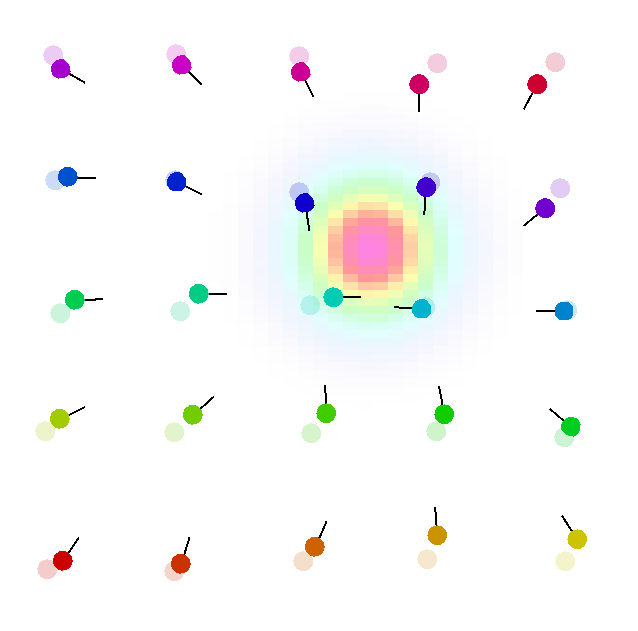
\includegraphics[width=\textwidth]{papers/acsos2023/imgs/start.png}
		\caption{Start}
		\label{acsos2023:fig:initial}
	\end{subfigure}
	\begin{subfigure}[b]{0.32\linewidth}
		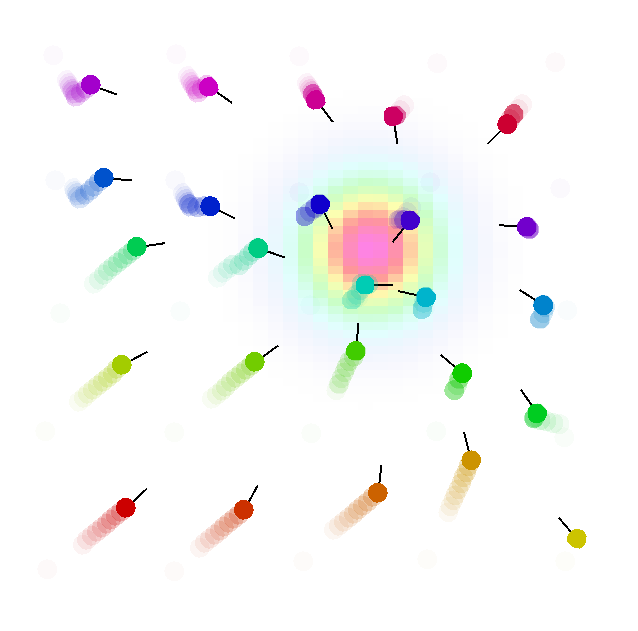
\includegraphics[width=\textwidth]{papers/acsos2023/imgs/after.png}
		\caption{After 50 steps}
		\label{acsos2023:fig:after}
	\end{subfigure}
	\begin{subfigure}[b]{0.32\linewidth}
		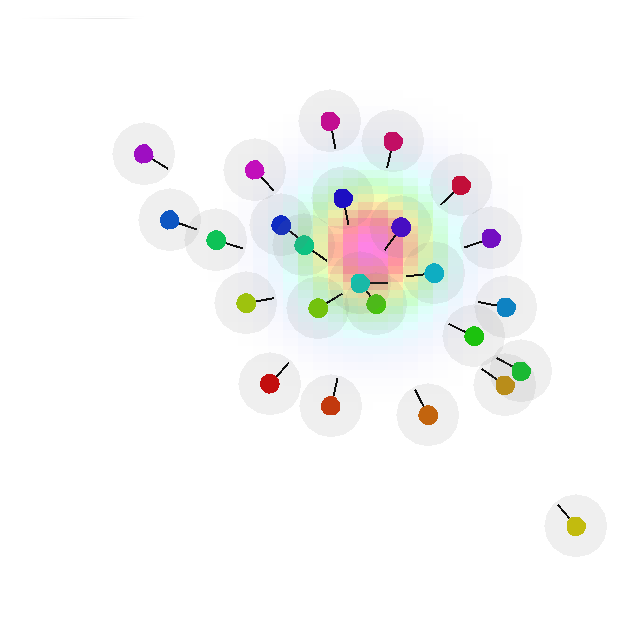
\includegraphics[width=\textwidth]{papers/acsos2023/imgs/end.png}
		\caption{After 200 steps}
		\label{acsos2023:fig:end}
	\end{subfigure}
	\caption[Phenomenon covering overview]{Agents (coloured dots) are deployed in an area and have to coordinate to cover the phenomenon. 
   The phenomenon can have varying areas of importance. 
   Over time, the phenomenon will be covered sufficiently without any central controller.
%		
%		Qualitative test results of the proposed approach. 
%		The agents go towards the phenomenon and try to cover it without collapsing into a single point.
%		the grey area represents the area covered by the agents (last figure on the right).
		}
	\label{acsos2023:fig:simulations}
\end{figure}

%Specifically, 
% our approach utilizes aggregate computing to disseminate information by manipulating a computational field, 
% which is a distributed data structure that maps devices to information. 
% This field functions as a dynamic environment in which information is continuously updated and diffused throughout the system. 
% By leveraging this layer, we can build collective distributed intelligence using \ac{GNN},
%  which uses the information in the field to determine the best action for a given task.
%\ga{first draft, need a refinement}
%The remainder of this paper is structured as follows. 
% First, we introduce the relevant background and problem formulation in \Cref{acsos2023:sec:background}. 
% Afterwards, we introduce our approach in \Cref{acsos2023:sec:approach}. 
% \Cref{acsos2023:sec:eval} outlines the performed experiments and discusses the obtained results. 
% Finally, we will present our conclusions in \Cref{acsos2023:sec:conclusion}.

\section{Background and Motivation}
\label{acsos2023:sec:background}
\subsection{Graph Neural Networks}

Graphs are ubiquitous structures that represent entities and their inter-relationships. With the rise of deep learning, there has been a growing interest in developing neural network models that can process graph-structured data. \ac{GNN} is one such model that has gained significant attention in recent years: it is a novel neural network model used to process graph-structured data with deep learning approaches. 
 Unlike traditional neural networks that operate on fixed-size vectors, \acp{GNN} are designed to handle irregular structures, 
 making them suitable for various applications where data is inherently graph-structured.

\subsubsection{Graph Representation}
Let $G = (V, E)$ be a graph where $E\subseteq V\times V$ defines the neighbourhood relations for each participating node, 
 and $V$ identifies the nodes present in the graph. 
 Each node $v \in V$ is associated with an observation (or feature set) $f_v$. For the sake of simplicity, 
 we thereafter describe $G_f$ as a graph that contains the feature set $f_v$ for each node $v \in V$. 
 Note that, when we refer to $G_f$ and $G_o$, 
 we are referring to the same graph $G$ but with different node features. 
 Also, to access the feature set $f_v$ of a node $v \in V$, we use the notation $f_v$ or $G_f[v]$.

\subsubsection{Objective of GNNs}

Given $f_v$, the goal of a \ac{GNN} is to learn the node embedding $h_v$ for each node $v \in V$. 
 The node embedding $h_v$ describes the node in the network and summarizes the geometric properties of the graph in this location, 
 allowing for comparison of various nodes in the graph. 
 This is analogous to how convolutional neural networks (CNNs) learn spatial hierarchies in images; 
 \acp{GNN} learn to capture the topological and combinatorial structure of graphs.

\subsubsection{Message Passing in GNNs}

In modern \acp{GNN}, the node embedding $h_v$ is computed by aggregating information from the node's neighbours $\mathcal{N}_G(v)$, and then combining it with the node's current embedding $h_v$ in a process called \emph{message passing}~\cite{DBLP:conf/icml/GilmerSRVD17}. This iterative process allows \acp{GNN} to capture long-range dependencies in the graph.

The \acp{GNN} is partitioned into several message passing layers $k$, where each of them is responsible for computing the node embedding $h_v^{(k)}$ for each node $v \in V$. Formally, a \ac{GNN} can be defined by three phases:

\begin{equation}
m^{(k)}_{uv} = \psi^{(k)}\left(h_u^{(k-1)}, h_v^{(k-1)}, e^{(k-1)}_{uv}\right) 
\end{equation}

\begin{equation}
a^{(k)}_u = \bigoplus^{(k)}\left(\left\{m^{(k)}_{uv}: v \in \mathcal{N}_G(u)\right\}\right)
\end{equation}

\begin{equation}
h_u^{(k)} = \phi^{(k)}\left(h_u^{(k-1)}, a^{(k)}_u\right)
\end{equation}

Where $h_{v}^{k}$ is the embedding of node $v$ within the $k$-th layer, and $\mathcal{N}_G(v)$ is the set of neighbours of node $v$ computed from $E$. The initial embedding $h_v^0$ is usually set to the node's feature vector $f_v$. The differential part comes into play in the $\psi$ and $\phi$ functions, which are typically differentiable functions such as neural networks.

\subsubsection{Aggregation Functions in GNNs}

The $\psi$ function, called the \emph{message function}, computes the message $m_{uv}^{(k)}$ from node $u$ to node $v$. The $\phi$ function, known as the \emph{update function}, updates the node embedding $h_v^{(k)}$ of node $v$. The aggregation function $\bigoplus$ aggregates information from the neighbours of a node $v$. While simple aggregation functions like sum, max, or sum of products are common, more complex aggregation functions have been proposed to capture intricate relationships in the graph~\cite{pellegrini2020learning}.

\subsubsection{GNN Application}

Applying a \ac{GNN} to a graph $G_f$ can be expressed as:

\begin{equation}
\mathit{GNN}(G_f) = \{h_v^{(k)}: v \in V, k \in \mathbb{N}\}
\end{equation} 

This formulation allows \acp{GNN} to effectively process and extract features from graph-structured data by iteratively aggregating and transforming information from the node's neighbours.

\acp{GNN} have found applications in diverse areas. They are used in social network analysis to understand user behaviours and community structures. In chemistry, they help in predicting molecular properties and drug discovery. In physics, they assist in understanding complex systems. In this chapter, we delve into the application of \acp{GNN} in multi-agent systems, focusing on learning local behaviours for each agent (more details in Section~\ref{acsos2023:sec:approach}).

\subsection{Problem formalization}
Given the homogeneity, large system scale, and the \emph{locality} (i,e., each agent can only observe its neighbours), 
 the problem can be modelled through the SwarMDP model~\cite{DBLP:conf/atal/SosicKZK17}---an extension of the \ac{DecPOMDP}~\cite{Decpomdp2000} model for swarm-like systems (see the \Cref{part:background} section for more details).
% 
However, In swarMDP, the neighbourhood is not directly defined, but it is implicitly defined by the observation model $\xi$.
In our specific case, the agents can only interact with 1-hop neighbours and are not directly influenced by other agent observations. We can therefore restrict the observation model as follows:
\begin{equation*}
\xi(v): \{s_j, j \in \mathcal{N}^v\} \rightarrow O
\qquad
\xi = \{\xi(v), v \in \mathcal{P}\}
\end{equation*}
where $\mathcal{N}^v$ is the set of neighbours of $v$.
%
This model can be used then to express the evolution of the system in time.
Specifically, starting from a global state $\mathcal{S}^P_t$, the next state $\mathcal{S}^P_{t+1}$ is defined as:
\begin{equation*}
\mathcal{A}^P_t = \pi(\xi(S^P_t))
\qquad
\mathcal{S}^P_{t+1} = \mathcal{T}(\mathcal{S}^P_t, \mathcal{A}^P_t)
\end{equation*}
Given a time $t$, the system can be also represented as a graph $G^t = {V^t, E^t}$, 
  where $E^t$ is built from $\mathcal{N}$.
  Each node is then decorated with the local observation perceived at the time $t$: $o^v_t \in O$. 
%
This graph can be used both to compute computational fields and, as done in previous work~\cite{DBLP:conf/corl/TolstayaGPP0R19,tolstaya2020learning,DBLP:conf/icra/GosrichMLPYR022}, can be the input for a GNN.
  % if we set $f_v = o^v_t$.
\subsection{Motivation}
Our work uniquely intersects the realms of automatic and manual methodologies, with a focus on field-based coordination and \ac{MAARL} empowered by \acp{GNN}.
%
Building upon foundational research in co-fields~\cite{DBLP:journals/pervasive/MameiZL04}, 
 we advance a novel framework where agents utilize a ``digital sign'' or computational field~\cite{DBLP:journals/ijaci/CastelfranchiPT10}. 
 This enables them to access and reason over global system data, 
 thereby enhancing their decision-making capabilities.

In our innovative model, 
 we integrate \ac{MAARL} and GNNs to foster agent intelligence. 
 This architecture allows agents to learn localized, yet comprehensive, representations of their surrounding environment.

Our approach diverges significantly from existing studies in which GNNs function as part of a distributed controller~\cite{DBLP:conf/icra/GosrichMLPYR022,DBLP:conf/corl/TolstayaGPP0R19}. 
 Although these works have demonstrated GNNs' utility in decentralized systems, they often relegate the communication aspect solely to neural networks. 
 This has been known to complicate and potentially destabilize the learning process.

In contrast, 
 our implementation ensures that the GNNs are guided by computational fields, narrowing the learning focus to specialized tasks as outlined by a collective reward function. 
 This design not only expedites learning but also enhances its stability.
\section{Field-informed Reinforcement Learning}
\label{acsos2023:sec:approach}
%\ga{Page budget: 2/3 pages \\}
%\ga{Plan: we should discuss the approach in detail, including the system model, and the learning dynamics. Particularly, I would like to highlight how each node in the graph is a local controller, but it could be seen as a global evolution, therefore we can use global information to inform the local controller.}
\begin{figure}
	\centering
  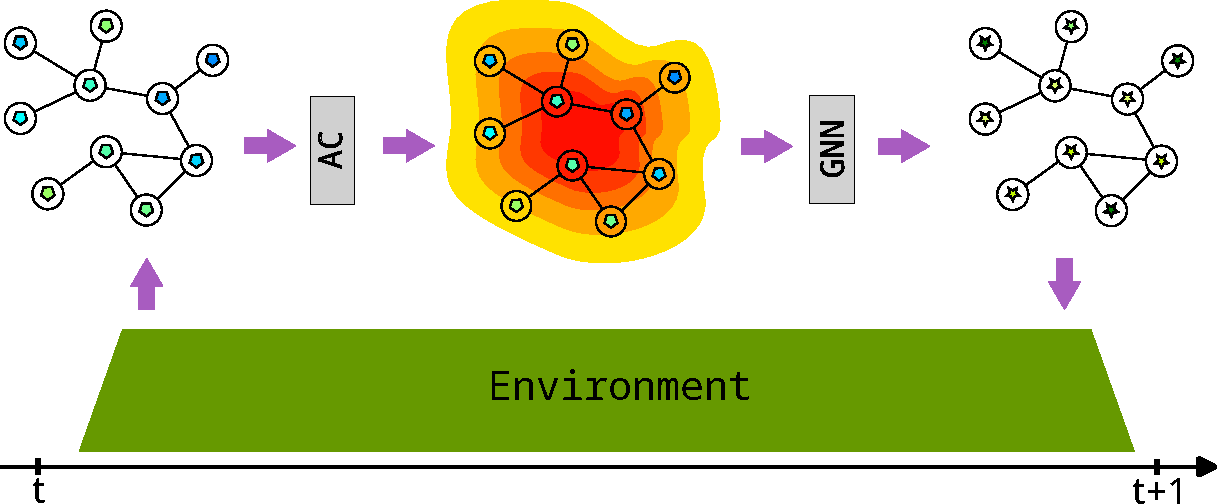
\includegraphics[width=.8\linewidth]{papers/acsos2023/imgs/architecture.pdf}

  \caption[High-level description of \ac{FIRL} approach.]{ High-level description of \ac{FIRL} approach. 
  For each time step $t$, a graph is constructed from the environment, and it will associate each node with a local feature $o^v_t$ (hexagons in the picture). 
  Using this feature, an aggregate program computes spatio-temporal information that enhances the feature set of each agent producing $f_v$, depicted as colours in the middle graph. 
  Finally, utilizing the GNN, actions are computed for each agent in the system to be performed against the environment, enabling advancement in the simulations according to swarMDP rules.
  %\lukas{should we have numbers at each step in the figure (and then referring in the caption and text)?}
  %\lukas{also, i think we can have the AC and GNN box a bit smaller but increase the size of the networks slightly - and put it on column width ot save space}
}  \label{acsos2023:fig:architecture}
\end{figure}
In this section, we discuss the components involved in our proposed solution---namely the \emph{architecture}---and how these components interact with each other to bring the system to perform the collective behaviour---namely the \emph{dynamics}. 
 Finally, we will detail the learning algorithm designed and used to synthesize the policy.
\subsection{Architecture, fields and aggregate dynamics}
%\ga{Plan: 
%  discussion about the typical AC evaluation model, specifying how GNN (with 1-hop information diffusion)
%  can be easily integrated with this distributed model
%}
The proposed solution, summarized in \Cref{acsos2023:fig:architecture}, consists mainly of two parts:
\begin{itemize}
  \item the aggregate program used to create part of the observation; 
  \item the policy $\pi_{gnn}$ learned through \ac{GNN}-based approach.
\end{itemize} 
%
Let $\Gamma$ be the aggregate program that takes a graph $G^t$ decorated by $o^v_t$, 
 representing the participating agents and their neighbourhood relations at time $t$, as input. 
%
The evaluation of $\Gamma$ produces a field value $\theta^v_t$ for each node $v$ in $G^t$. 
From this field, we construct the feature vector $f_v$ for each node $v$ in $G^t$ as follows:
 $f_v = (\theta^v_t, o^v_t)$.
%
The policy $\pi_{gnn}$ is then evaluated for each agent using $f_v$ as input, 
 producing an action $a^v_t$ that will then modify the global state of the system.
 %\ga{todo: put pseudo code to express this dynamics}
%
While the graph, containing the aggregate information, 
 might appear as global knowledge, 
 this is not the case as the information is \emph{never} aggregated globally. 
The individual agents only combine information from their local neighbourhood.
%
In fact, the program $\Gamma$ is proactively executed at every agent, 
and the \ac{GNN} can be locally evaluated using only neighbourhood information. 
%
We want to emphasize that, in this case, the \acp{GNN} must be 1-hop; 
otherwise, they could not have a local interpretation for each agent, according to our system model.
\subsection{Learning algorithm}
%
Since we consider swarm-like systems, 
 which are an example of many-agent systems, 
 the proposed approach follows a \ac{CTDE} learning pattern,
 but differently from mean-field approaches and actor-critic solutions,
 we use a \emph{value-based} approach combined with a \ac{GNN} as a function approximator.
%
Specifically, we leveraged the property of \acp{GNN} to have a \emph{dual} interpretation, 
i.e., to function globally over the entire graph and locally only over the neighbourhood. 
Importantly, each agent only has local information from itself and its neighbourhood to utilize in the \ac{GNN}.
%
As value-based algorithm we relied on \ac{DQN}~\cite{mnih2015playing} 
with two major modifications (see \Cref{chap:rl:single}): 
\begin{enumerate}
  \item experience replay stores experiences in the form of \emph{graphs} decorated with features (e.g., observations, actions, rewards, etc.),
  \item the neural network used to compute the Q function is based on a \ac{GNN} with an \ac{MLP} downstream.
\end{enumerate}
The first point is a natural extension because we work on graphs rather than simple values.
This also influences how we create a batch of experiences to train the network.
 In fact, we sample a batch of graphs from the replay buffer,
 and then we merge them into a single graph,
 which is then used to train the network.
 This process is called \emph{graph mini-batching}~\cite{DBLP:journals/corr/abs-1903-02428,wang2019deep}
 and its main purpose is to pass an entire batch of graphs to the same \ac{GNN} for improved performance.
%
For the second point,
 the use of \acp{GNN} allows us to define policies on a variable neighbourhood, which is essential in such systems as this can change due to the applied neighbourhood policy.
 It is known that \acp{GNN} have a certain ability to generalize to new structures and scale with different agents~\cite{DBLP:journals/aiopen/ZhouCHZYLWLS20,DBLP:conf/nips/KnyazevTA19}. 
% 
Additionally, 
 using the overall graph compared to local experiences makes learning more stable as it reduces the non-stationarity of the environment perceived by each node.
% 
This is because, even though the actions are produced using only local and neighbourhood information, 
 during the learning phase, we have access to the internal graph, 
 which will influence the policy through non-local information 
 during the backpropagation.
%
\begin{algorithm}
  \KwIn{Environment $\mathbb{E}$, graph replay buffer $\mathcal{D}$, target network $\theta^{-}$, current network $\theta$, exploration strategy $\epsilon$}
  \KwOut{Trained DQN model $\theta$}

  Initialize $\mathcal{D}$ with random initial transitions;

  Initialize $\theta$ with random weights;

  Set $\theta^{-} \leftarrow \theta$;

  \While{not done}{
  Observe current graph observations $G_o$;

  \uIf{random $< \epsilon$}{
    select a random action $a$;
  }
  \Else{
    $G_q = Q(G_o, \theta)$;
    $a = \{ v \in G_q | a_v \in argmax_{a_v} G_q[v](a_v) \}$;

  }

  Execute the collective action $G_a$ in the environment $\mathbb{E}$ and observe a graph-level reward $G_r$ and the next observation $G_o'$;

  Store transition $(G_o,G_a,G_r, G_o')$ in $\mathcal{D}$;

  Sample a batch of graph transitions $(G^i_o,G^i_a,G^i_r,G'^i_o)$ 
   from $\mathcal{D}$ and merge them in $(G^b_o,G^b_a,G^b_r,G'^b_o)$; 

  Compute the target Q-value for each node $v$ in the graph $G^b$: 
  $y_v = G^b_r[v] + \gamma * \max{a'} Q(G'^b_o[v],G^b_a[a'];\theta^{-})$;
  
  Compute the current expected value for each node $v$ in the graph $G^b$:
  $y_v^* = Q(G^b_o[v],G^b_a[v];\theta)$;

  Update the current network weights using gradient descent: $\theta \leftarrow \theta - \alpha \nabla{\theta} \frac{1}{|G^b|} (y - y^*)^2$;

  Every $C$ steps, update the target network weights: $\theta^{-} \leftarrow \theta$
  ;
  }
  \caption{Deep Q-Network (DQN) with GNN and Graph Replay Buffer executed by each agent}
  \label{acsos2023:alg:dqn}
  \end{algorithm}
 
    
\section{Evaluation}
\label{acsos2023:sec:eval}
\begin{figure}
  \centering
  \begin{subfigure}[b]{0.32\linewidth}
      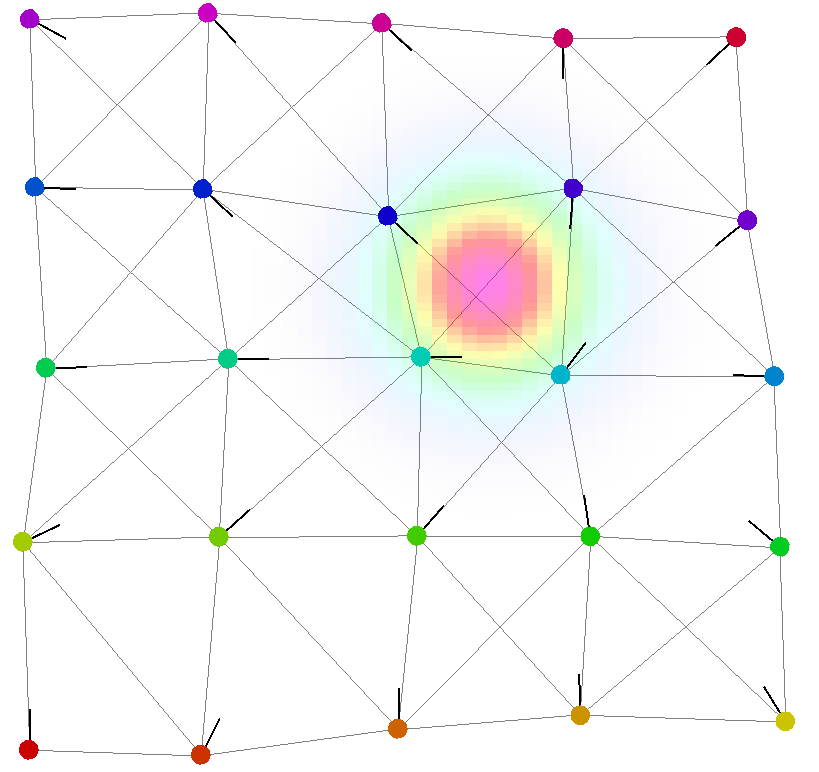
\includegraphics[width=\textwidth]{papers/acsos2023/imgs/example.png}
      \caption{}
      \label{acsos2023:fig:static}
  \end{subfigure}
  \begin{subfigure}[b]{0.32\linewidth}
      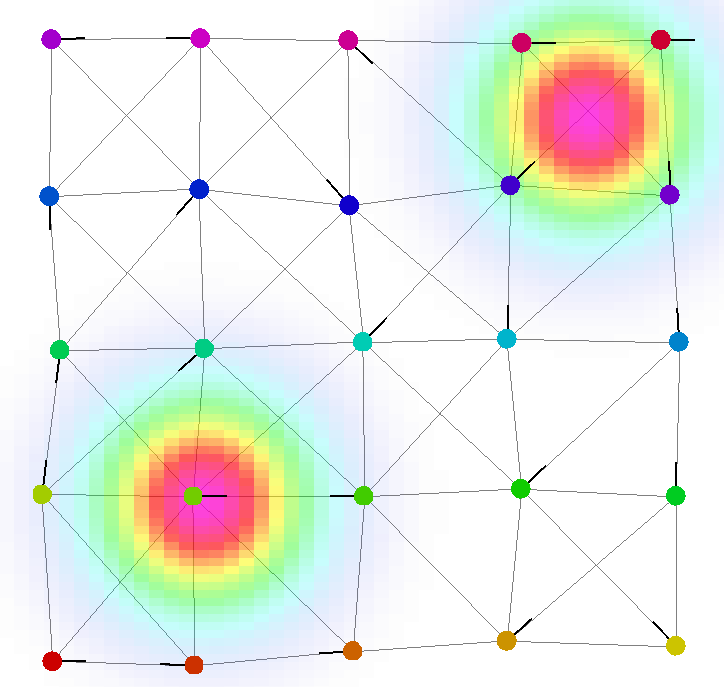
\includegraphics[width=\textwidth]{papers/acsos2023/imgs/two-zones.png}
      \caption{}
      \label{acsos2023:fig:two}
  \end{subfigure}
  \begin{subfigure}[b]{0.32\linewidth}
      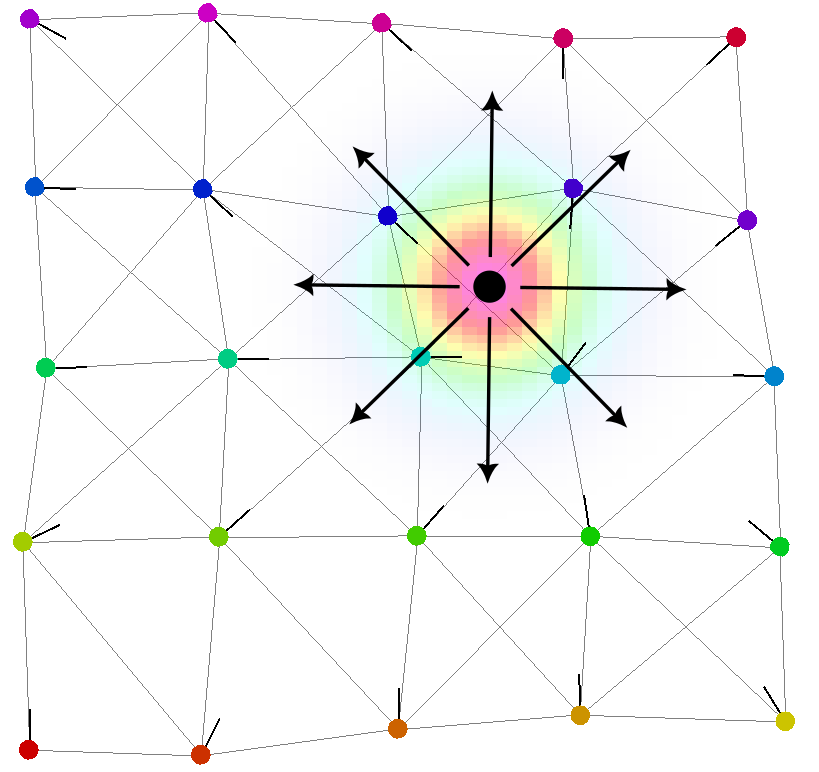
\includegraphics[width=\textwidth]{papers/acsos2023/imgs/example-moving.png}
      \caption{}
      \label{acsos2023:fig:moving}
  \end{subfigure}

  %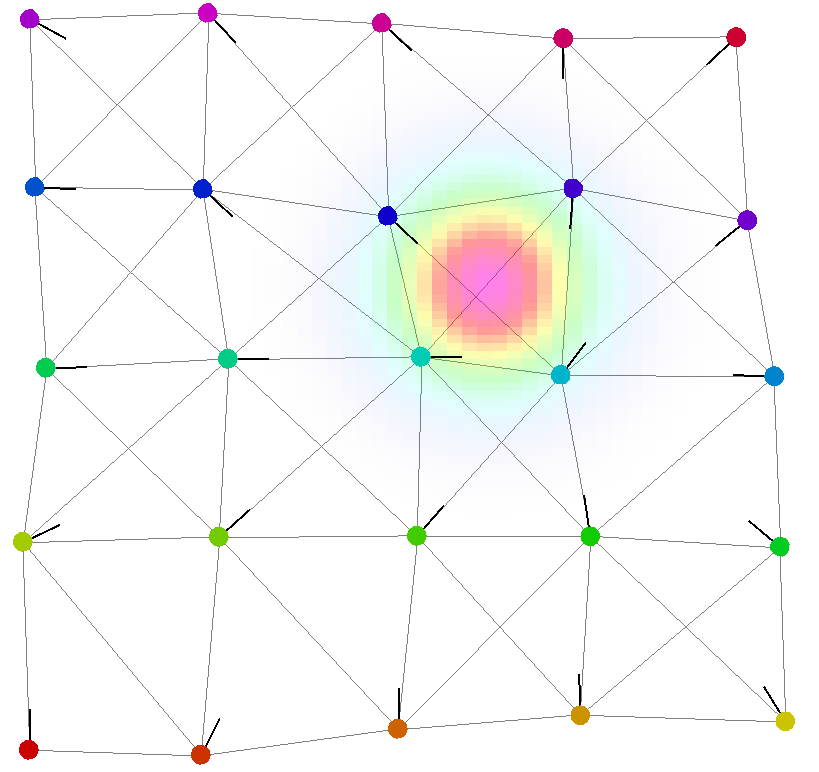
\includegraphics[width=0.3\textwidth]{papers/acsos2023/imgs/example.png}
 
  \caption[Simulations of the case study scenario in Alchemist for \ac{FIRL}.]{Simulations of the case study scenario in Alchemist. 
  The dots represent drones, 
  the circle area on represents the phenomenon to be monitored.
  \Cref{acsos2023:fig:static} represents the scenario used during training \review{as well as during test}. 
  The others \review{instead} are only used in the test phase to evaluate the policy found. }
  \label{acsos2023:fig:scenarios}
\end{figure}
To test the effectiveness of the proposed approach, 
 we experiment with a case study related to swarm robotics leveraging Alchemist, 
 specifically, tracking and coverage of a spatio-temporal phenomenon---cf. tracking a wildfire 
 or monitoring the water levels in a canal with multiple autonomous drones embodied in embedded devices (e.g., drones or IoT devices)---similar to the ones discussed in \Cref{part:background}. 
 The individual drones do not have any knowledge of the initial phenomenon itself (i.e., shape, size, location, velocity, and so on).
 %
Initially, 
  we perform the training phase using a stationary phenomenon before expanding towards a moving phenomenon in the test phase. 
  %Additionally, the phenomenon can change its shape during runtime. 
  Finally, the phenomenon may have varying areas of interest, defined by an underlying distribution function. 
  This underlying distribution is utilized in the feature set of each drone's observation and guides the drones to rally over the phenomenon. 
  While we only use Guassian distributions but we can use any other distribution and shape. 
For the \ac{GNN}, we use the implementation provided by PyTorch Geometric~\cite{Fey/Lenssen/2019}, 
 which is a library for deep learning on graphs built on top of PyTorch~\cite{torch}.
Finally, we use \scafi{}~\cite{casadei2022scafi} as the aggregate programming language to support our field-informed approach.
%
The evaluation is performed in two stages, 
 first the neural networks are trained in an explicit training phase before being extensively evaluated in the testing stage.
\footnote{The simulations are publicly available at \url{https://github.com/AggregateComputing/experiment-2023-acsos-field-informed-rl}.}
\subsection{Scenario}
\Cref{acsos2023:fig:scenarios} presents the three different types of scenarios utilized within the evaluation. 
 The first type of experiments considers a single phenomenon at a static location (i.e., \emph{Zone Fixed}), 
 the second type of experiment considers two phenomena in two independent but static locations (i.e., \emph{Two Zones}), 
 and the third type of experiment considers a moving phenomenon (i.e., \emph{Moving}). 
 All phenomena are modelled as a Gaussian distribution. 
 Importantly, only the left scenario illustrated in Figure~\ref{acsos2023:fig:static} was used for training the neural networks. 
Furthermore, all three types of scenarios contain a set of $\mathcal{P} = 25$ drones placed in a 2D grid large 1000x1000 meters. % and a single, stationary phenomenon with a  
Each drone can perceive the presence
 of the phenomenon of interest through an installed sensor $\zeta_v$ with $v \in \mathbb{V}$. 
 (e.g., camera, temperature sensor, etc.) if it is within range.
%
Additionally, each drone has a coverage range $\omega$ (fixed to 75 meters) 
 that describes the area it can monitor. 
 Each drone can only communicate directly with its own neighbourhood $\mathcal{N}$, 
 which in this case depends on a $\mathbb{O}$ range fixed to 300 meters. %\lukas{$\mathbb{O}$  not defined.}
Through this communication channel, drones can exchange information. 
%From the neighbourhood, each agent can also perceive the direction of the other agents.
%
Each drone moves following a certain action composed of two components (r, i) 
 which respectively describe the angle and intensity of the movement (i.e., the velocity vector).
Since we used a value-based approach, 
 the action space $\mathcal{A}$ is discrete and composed of 18 possible angles and 3 possible intensities.
In particular, the angles are quantized to 20 degrees, and for the velocities, we have selected [0, 5, 10] m/s.
%\lukas{is this training the \ac{GNN}? }, 
%

For the aggregated information, each drone will produce a computation field with which they will try to approximate the direction of the phenomenon of interest. 
%
%
%The specific program in question is a simple application of block G, where the source is the maximum value of the neighbourhood. 
The program $\Gamma$ in question is a simple application of block \lstinline|G|, where the source is the maximum value of the neighbourhood. 
This can be expressed in \scafi{} as follows:
\begin{lstlisting}[mathescape=true]
val source = maxHood(nbr(sense($\zeta$))) == sense($\zeta$)
G(source, Point3D.Zero, _ + nbrVector())
\end{lstlisting}
where \texttt{maxHood} is a function that returns the maximum value of the neighbourhood, 
 \texttt{nbr} is a function that a neighbourhood field of values (in this case, the sensor value $\zeta$),
\texttt{sense} is a function that returns the value of the sensor, and
\texttt{nbrRange} is a function that returns an approximate direction for each drone in the neighbourhood.
%
This value will then be fed into the $\pi_{GNN}$ to compute the action to be performed.
\subsection{Goal}
 The objective of this scenario is threefold:
\begin{enumerate}
\item maximize the number of drones within the phenomena;
\item minimize the number of drones without neighbours;
\item maximize the coverage of the system.
\end{enumerate}
As we are modelling a reinforcement learning system, 
 these three components must be encoded in a reward function 
 that provides an estimate of the current action taken by a given drone.
% 
% Regarding the first point, the reward function is simple and is defined as:
Formally, we define the reward of a drone being within the phenomenon as:
\begin{equation}
R^a_{v} = 1 \text{ if } \zeta_v > 0 \text{ else } 0  
\end{equation}
Namely, a drone is considered within the phenomena as soon as the drone can sense the phenomenon.
%
This will lead the system to prefer a configuration in which every drone is present within the phenomenon.
%
The second element in the objective function ensures cohesion among the drones. 
 This is important because if the system breaks into many scattered drones, 
 the observability of the phenomenon is reduced, 
 limiting the ability of the drones to move appropriately in the environment.
% they are not able to move in the environment due to the reduced observability of the system. 
 In this case, the reward is defined as:
\begin{equation*}
R^{\mathcal{N}}_{v} = 1 \text{ if } |\mathcal{N}| > 0 \text{ else } 0
\end{equation*}
Finally, to maximize the coverage, 
  we define a reward function that favours the maximum distance between the drones
  equal to the coverage range $\omega$. 
  This will minimize multiple drones covering a common area.
%
This means that the average distance will tend towards the one expressed by the viewing range of each drone:
% 
\begin{equation*}
R^{C}_{v} = 1 - \frac{d_{min}}{\omega}
\end{equation*}
Where $d_{min}$ describes and minimum distance of the drone to its neighbourhood. 
%
%\lukas{should this be $1-R^C_v$? or do we want to favour the highest average distance?}
The final reward function $R_{v}$ for an agent $v$ is defined as:
\begin{equation*}
 R_{v} = (\frac{R^a_{v} + R^{\mathcal{N}}_{v} + R^{C}_{v}}{3}) - 1  
\end{equation*}
Specifically, we decided to express the signal as a \emph{regret}
  as it is a more general measure of the quality of the action taken by the drone.
%
\subsection{Training Phase}
Before we can evaluate our approach, the underlying neural networks have to be fine-tuned in a dedicated training phase.
The training process for each neural network was divided into 100 episodes, each consisting of 200 steps, resulting in a total of 20,000 experiences.
%
For each episode, 
 the 25 drones are semi-randomly positioned on a grid (i.e., in a lattice layout with a random variation in their position) without knowing the correct position of the phenomenon, 
 but that is fixed in the top right corner. 
 The position of the phenomenon with an example of positioned drones can be seen in Figure~\ref{acsos2023:fig:static}. 

 The feature set used by the \ac{GNN} created for each drone consists of the vector computed by the aggregated program and the value of the local sensor $\zeta$.
%
In this case, we chose to use an exponential epsilon decay, defined as:
$$\epsilon = \epsilon_{min} + (\epsilon_{max} - \epsilon_{min}) \cdot e^{-\lambda \cdot e}$$
Where $e$ is the current episode number. 
This leads to a high number of random actions at the beginning and gradually shifts towards exploitation in the later episodes. 
%
In our training process, 
 we set $\epsilon_{min} = 0.02$, $\epsilon_{max} = 0.99$, and $\lambda = 0.1$.
$\gamma$ was set to 0.99, 
 as we want to give more value to future returns, 
 aiming to achieve good coverage by continuously tracking the phenomenon. 
The neural network structure used consists of a layer of SuperGAT~\cite{DBLP:journals/corr/abs-2204-04879} ---a \ac{GNN} based on attention mechanisms--- and a layer of MLP. 
The hidden size was set to 256.
%
As the reward function is defined as a regret, 
 we decided to use the Huber loss function with $\delta = 1$. %~\cite{??}, 
 which is a combination of the $L_1$ and $L_2$ loss functions:

\begin{equation*}
L_\delta = \begin{cases}
  \frac{1}{2} (y - \hat{y})^2 & \text{if } |y - \hat{y}| < \delta \\
  \delta \cdot (|y - \hat{y}| - \frac{1}{2} \delta) & \text{otherwise,} 
 \end{cases}
\end{equation*}
where $\delta$ is a hyperparameter that determines the threshold between the two loss functions (fixed to 1 in our experiemnt) and $y$ and $\hat{y}$ are the target and predicted values, respectively.
This function is used to penalize the drone if the action taken is too far from the optimal action. 
%\lukas{what is the value of $\delta$ in the training?}
%\lukas{also: $\delta$ is used as a function and as a value?}
%
We use the RMSprop optimiser with a learning rate of 0.0001.
%
Finally, we use a replay buffer of size 1000 to store the graph experiences and a batch size of 32.
\subsection{Test phase}
For the evaluation, 
 we explore the previously discussed three different types of experiments.
%
We generated 64 random scenarios for each type of experiment. 
 Additionally, the placement of the drones was randomized as it has been done during training.
For the first type, consider a single static phenomenon randomly placed in the environment. 
This is in contrast to the training where the phenomena were always placed in the same location.  
For the second type, we placed two distinct phenomena within the area. 
Their location is kept constant in all 64 experiments. 
As the training only contained a single phenomenon, 
this setup represents a challenge for the drones.
Finally, the third type contained moving phenomena. 
In each scenario, the starting position as well as the direction of movement is randomly sampled from a uniform distribution. 
The movement is in a straight line with a constant speed of 5m/s within an unbounded environment. 
%to ensure the agents can keep up with the phenomenon. 
%\lukas{64 experiments per mode with random initial positions of the phenomena. Moving: starting at random position and move in a straight line moving with 5m/s in an unbounded environment.}
%
Examples of all three types of experiments are shown in~\Cref{acsos2023:fig:scenarios}. %\lukas{can we create a figure with at least 3 sample scenarios (1 stationary, 2 split, 1 moving (with a line indicating its trajectory))?} 

%\lukas{I would move this up into IV.A --> emphasise that we only used a single static phenomena in the training therefore this section is improtant!}

\subsection{Baselines}
We compare our \ac{FIRL} approach against baseline approaches where the \ac{DQN} utilizes a \ac{MLP} as well as an approach only relying on \acp{GNN}, without additional field information. 
%
In all approaches, the underlying neural network (i.e., the \ac{MLP} and the \ac{GNN}) are trained %with the same parameters of the proposed approach 
with a single, stationary phenomenon.
%

The \ac{MLP} uses the same feature set as the \ac{GNN} but applies it in the \ac{DQN} but 
%in the proposed approach, but differently, it uses a standard DQN approach 
without leveraging the graph structure. Moreover, we increase the batch size to 512 and the replay buffer to 10000 since we record 25 drones' experiences for each step instead of one graph experience.
%\lukas{to make sure: in all three cases we use DQN but with (i) MLP, (ii) standard GNN, (iii) our approach - a field-informed GNN, right?}
%
%The \ac{GNN} instead of using the field information, use directly the position of nodes and the local sensor value as input features.
The \ac{GNN} alone, without using the field information, apply the position of drones and the local sensor value directly as input features within the \ac{DQN}.
%
These baselines are used to verify the effectiveness of the components used in the FIRL. 
%
Indeed, the \ac{MLP} baseline is used to verify the effectiveness of the \ac{GNN} in the proposed approach, while the \ac{GNN} baseline is used to verify the effectiveness of the field information in the proposed approach.
\subsection{Metrics}
We evaluate the performance of the different approaches by measuring the coverage of the phenomenon over time.
%
The coverage is defined as the percentage of the phenomenon covered by the drones.
%
Specifically, we can measure the coverage as the intersection over the union of the phenomenon and the drones' view range.
%
Formally, we define the overall coverage for a certain time step as:
\begin{equation*}
\Omega = \bigcup_{v \in V} \omega_v
\quad 
C = \frac{|\Omega \cap \mathcal{P}|}{|\mathcal{P}|}
\end{equation*}
where $\mathcal{P}$ is the area of the phenomenon and $\Omega$ is the area covered by the drones.
%This is computed for each step of the simulation. 45
In the training phases, 
 we measure the average coverage in each episode, and the total reward obtained by the drones at each episode of the simulation. 
%
We also measure the number of drones that are within the phenomenon at each step of the simulation.
This will be a measure of how well the drones are tracking the phenomenon.
%\ga{todo improve the description of the coverage}

\subsection{Discussion and Results}
The results of the training process are summarized in \Cref{acsos2023:fig:training}.
% 
\review{In the charts, the line represents the average value of a metric of interest, while the shaded area represents its standard deviation.}
%
Specifically, we observe that the proposed version achieves higher coverage and total reward compared to other approaches. 
%
Interestingly, despite the global information available in \acp{GNN} without fields, they fail to converge to a good result like the one obtained with the field. 
%
This outcome was expected, as the computed field helps drones encode the necessary information to navigate towards the phenomenon.
%
Furthermore, we note that \ac{GNN} combined with \ac{DQN} and graph replay buffer outperforms the simple \ac{MLP} informed field computation. 
%
This is because relying solely on \ac{MLP} and basic deep learning leads to non-stationary and unstable learning, 
 as evident from the wider confidence interval of the reward over training time.

Focusing now on the results of the test phase, highlighted in  \Cref{acsos2023:fig:test},
 we observe that the field-informed version achieves higher coverage than the other approaches in all scenarios since it shows the ability of our solution to generalize to situations. 
% 
We observe that the field-informed version successfully moves the drones closer to the target phenomenon, 
 distributing them evenly without collapsing into a single central point. 
 \Cref{acsos2023:fig:test} quantitatively presents the results across various previously described scenarios.

For all experiments, both \ac{GNN} versions demonstrate the capability to transfer the learned experience to the test phase whereas the MLP version fails to generalize. 
%
It is worth noting that, in the \emph{Zone Fixed} experiment, % (left graph in \Cref{acsos2023:fig:test}), 
 once the desired configurati45on is achieved in the static case, 
 the drones cease to move, maintaining the found configuration.
%
Interesting observations arise when we use scenarios different from the training phase. 
% Starting from a division into two zones, 
In the \emph{Two Zones} experiment,
 we notice that our approach using field-information finds a better configuration than the simple GNN counterpart. 
%
It exhibits both higher overall coverage and manages to divide the system into two equally covered parts. 
%
Indeed, observing the \Cref{acsos2023:fig:resCoverage}, we notice that the informed version maintains a balanced coverage between the two zones, 
 with a difference of less than 5\% between the two parts, maintaining a fair division of the phenomena.
%
In contrast, the uninformed version also maintains a fair division but with significantly different coverage between the two parts, 
 indicating a wrong placement among the drones in one of the zones.
%
This is a consequence of the uninformed version's inability to encode the necessary information to divide the drones into two zones, therefore it is not able to generalize.
%
Finally, the \emph{Moving} experiment emphasizes how the informed version generates a more robust policy for new scenarios. 
 Indeed, we observe that our approach using \ac{FIRL} maintains higher coverage and a greater number of drones on the target phenomenon compared to the other two solutions.
%
The uninformed GNN version, however, 
 fails again to generalize its movement behaviour, as evidenced by the simulations where the drones, once reaching the target zone, stop moving due to tracking issues.

In conclusion, the results demonstrate how the proposed idea can generate more robust controllers. 
 By guiding information flow in \acp{GNN}, 
 we improve learning efficiency and alleviate the challenge of encoding relevant information. 
%
Nevertheless, we acknowledge the crucial role of \acp{GNN}. 
 Our modified version of DQN, combined with \acp{GNN}, 
 enables the discovery of robust behaviours in a few episodes, 
 which is challenging to capture with \acp{MLP} combined with \ac{DQN}, even if we use field information.
% \lukas{add short discussion on 'new' figure 6}
\begin{figure}
  \centering
  \hfill
  \begin{subfigure}[b]{0.45\linewidth}
    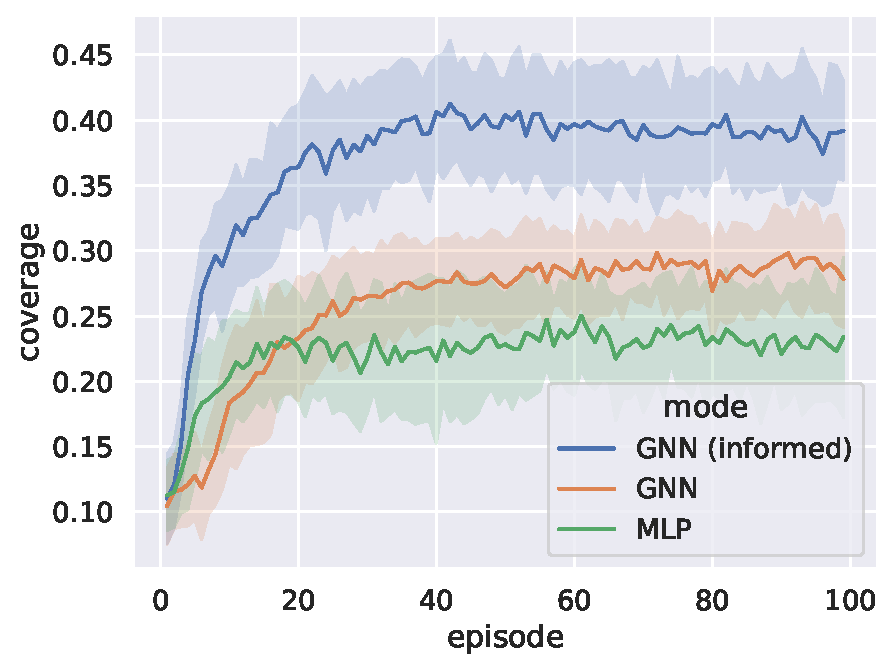
\includegraphics[width=\linewidth]{papers/acsos2023/imgs/coverage-in-time}
    \caption{Average coverage for each episode in training }
    \label{acsos2023:fig:coverage}
  \end{subfigure}%\\
  %\hfill
  \begin{subfigure}[b]{0.5\linewidth}
    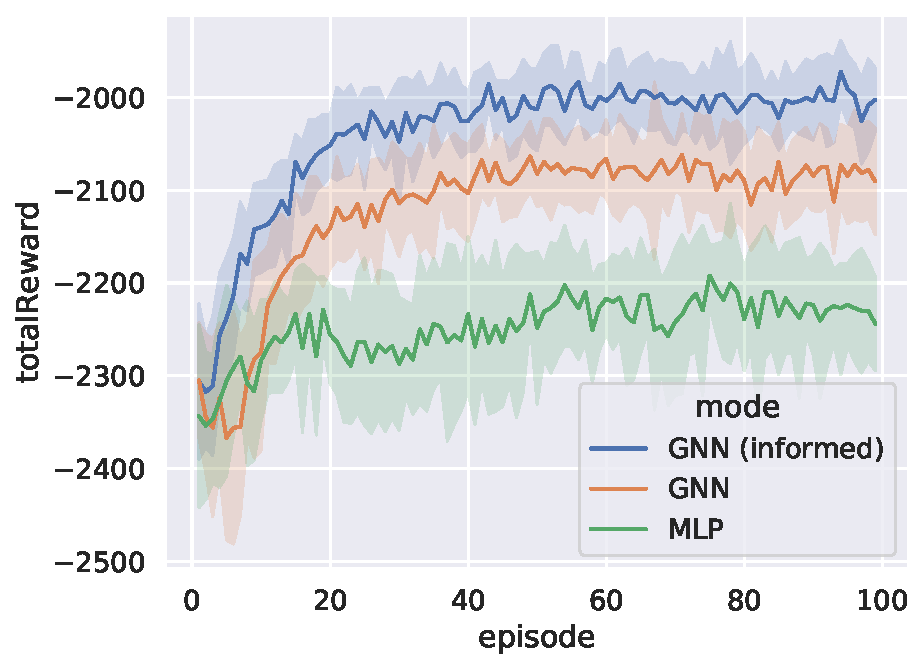
\includegraphics[width=\linewidth]{papers/acsos2023/imgs/reward-in-time}
    \caption{Reward during training}
    \label{acsos2023:fig:reward}
  \end{subfigure}
  \caption[Training results of \ac{FIRL}.]{Training results of \ac{FIRL}.
  It can cover the phenomenon better than the baselines, and it reaches a higher reward. 
  }
  \label{acsos2023:fig:training}
\end{figure}


%% Create a subfigure of coverage-test, inside-test, inside-two-test and coverage-two-test

\begin{figure*}
  \centering
  \begin{subfigure}[b]{0.75\linewidth}
    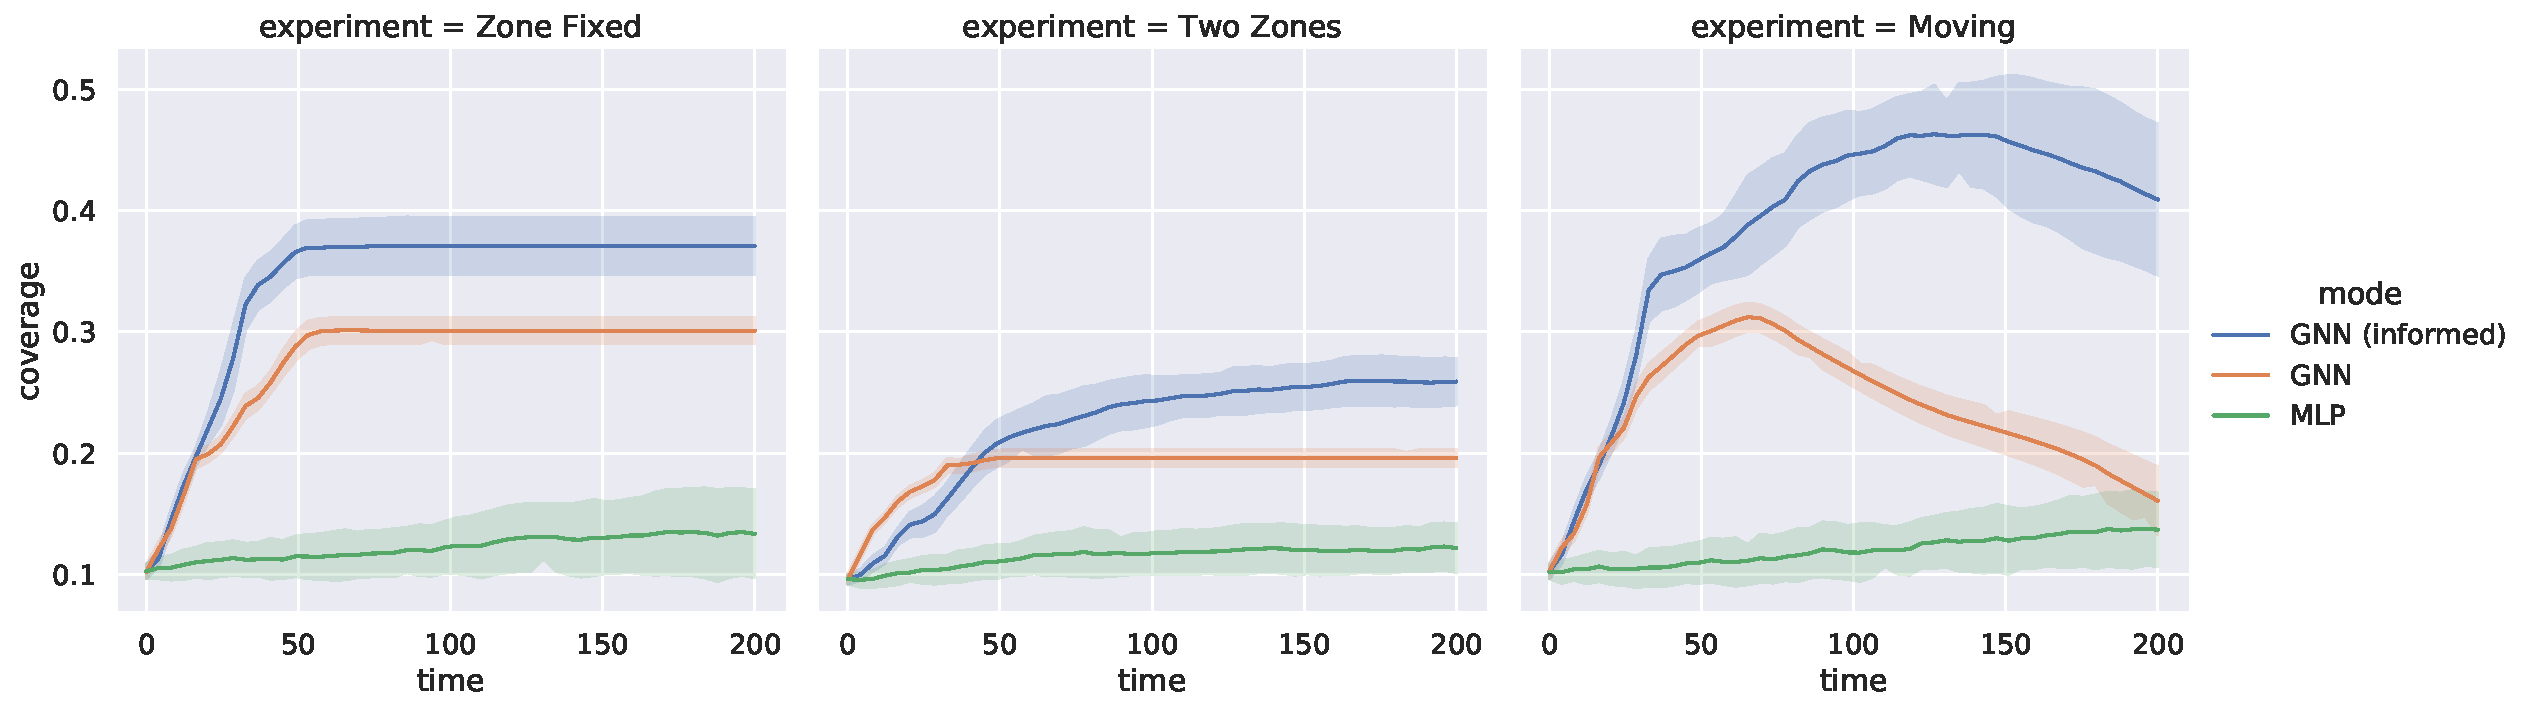
\includegraphics[width=\linewidth]{papers/acsos2023/imgs/coverage-test.pdf}
    \caption[Ratio of coverage of the phenomena in \ac{FIRL}]{Ratio of coverage of the phenomena. Our \ac{FIRL} approach can outperform other approaches lacking field information.}
    \label{acsos2023:fig:coverage-test}
  \end{subfigure}
  \begin{subfigure}[b]{0.75\linewidth}
    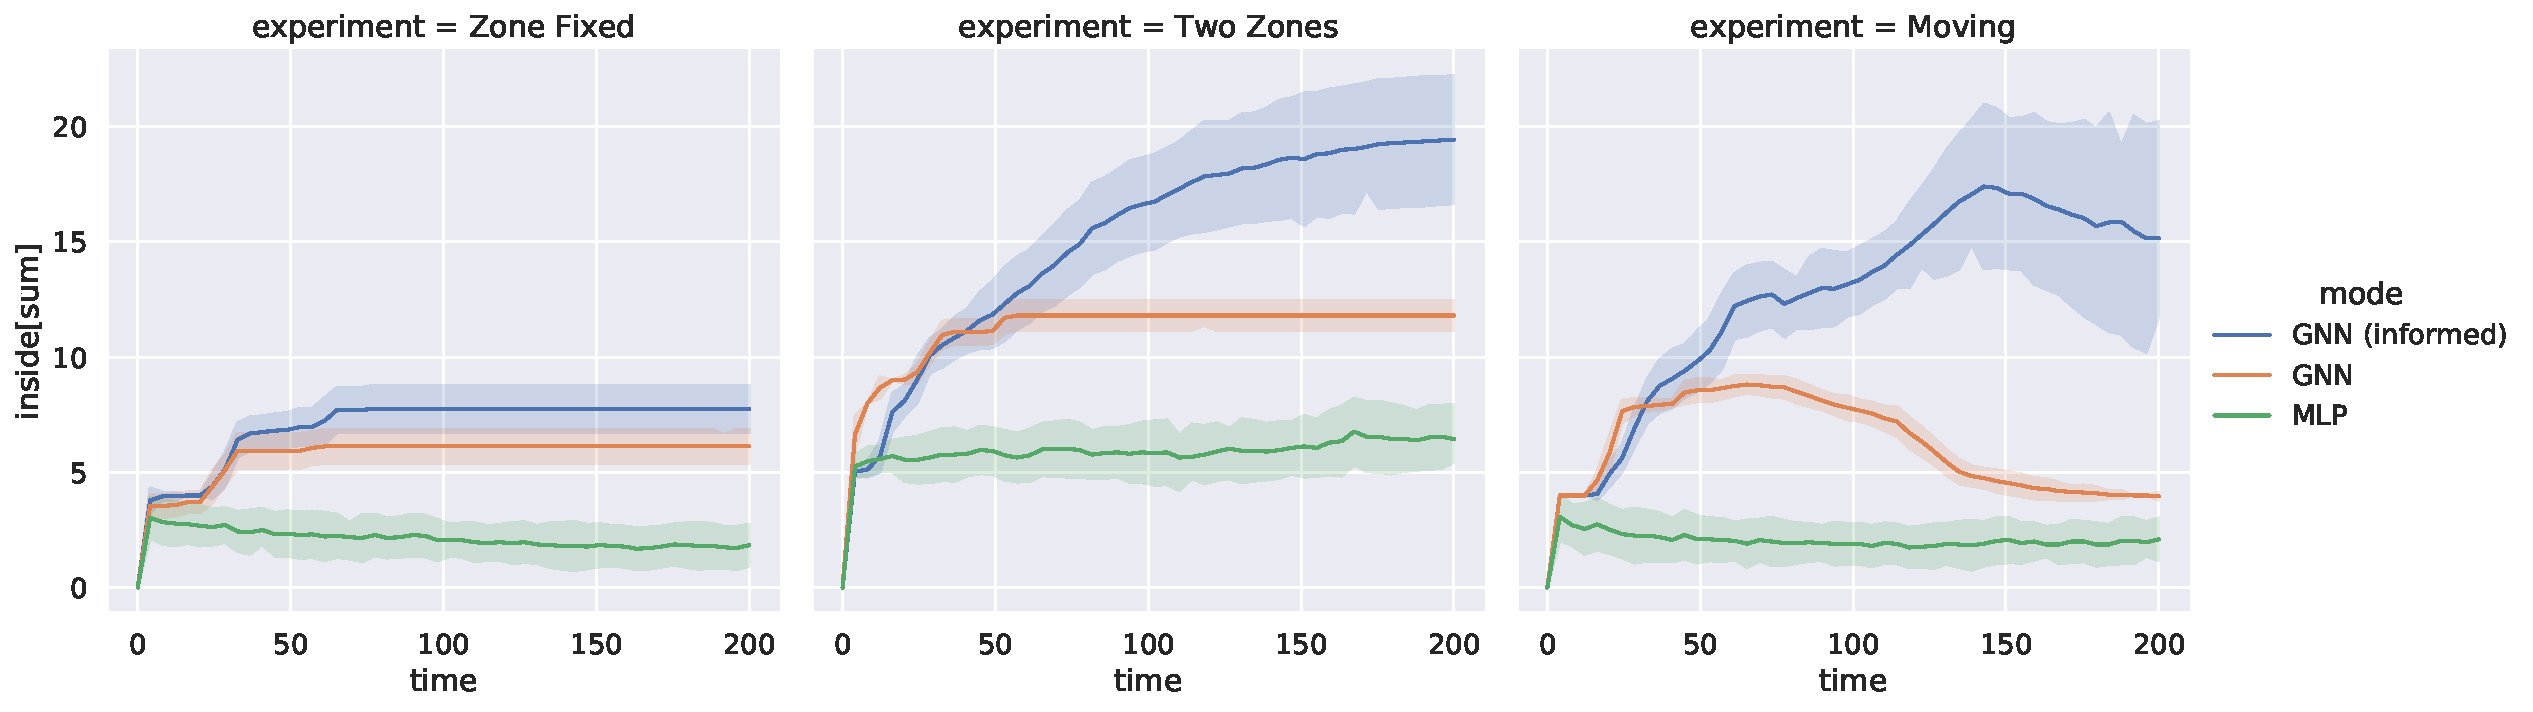
\includegraphics[width=\linewidth]{papers/acsos2023/imgs/inside-test}
    \caption{Number of drones inside the phenomenon in the three types of experiments}
    \label{acsos2023:fig:inside-test}
  \end{subfigure}
	\caption[Quantitative test results of \ac{FIRL}]{Quantitative test results.
	 	The proposed approach can cover and track the phenomenon better than the baselines.
	}
	\label{acsos2023:fig:test}
\end{figure*}
\begin{figure*}
	\centering
  	\begin{subfigure}[b]{0.75\linewidth}
    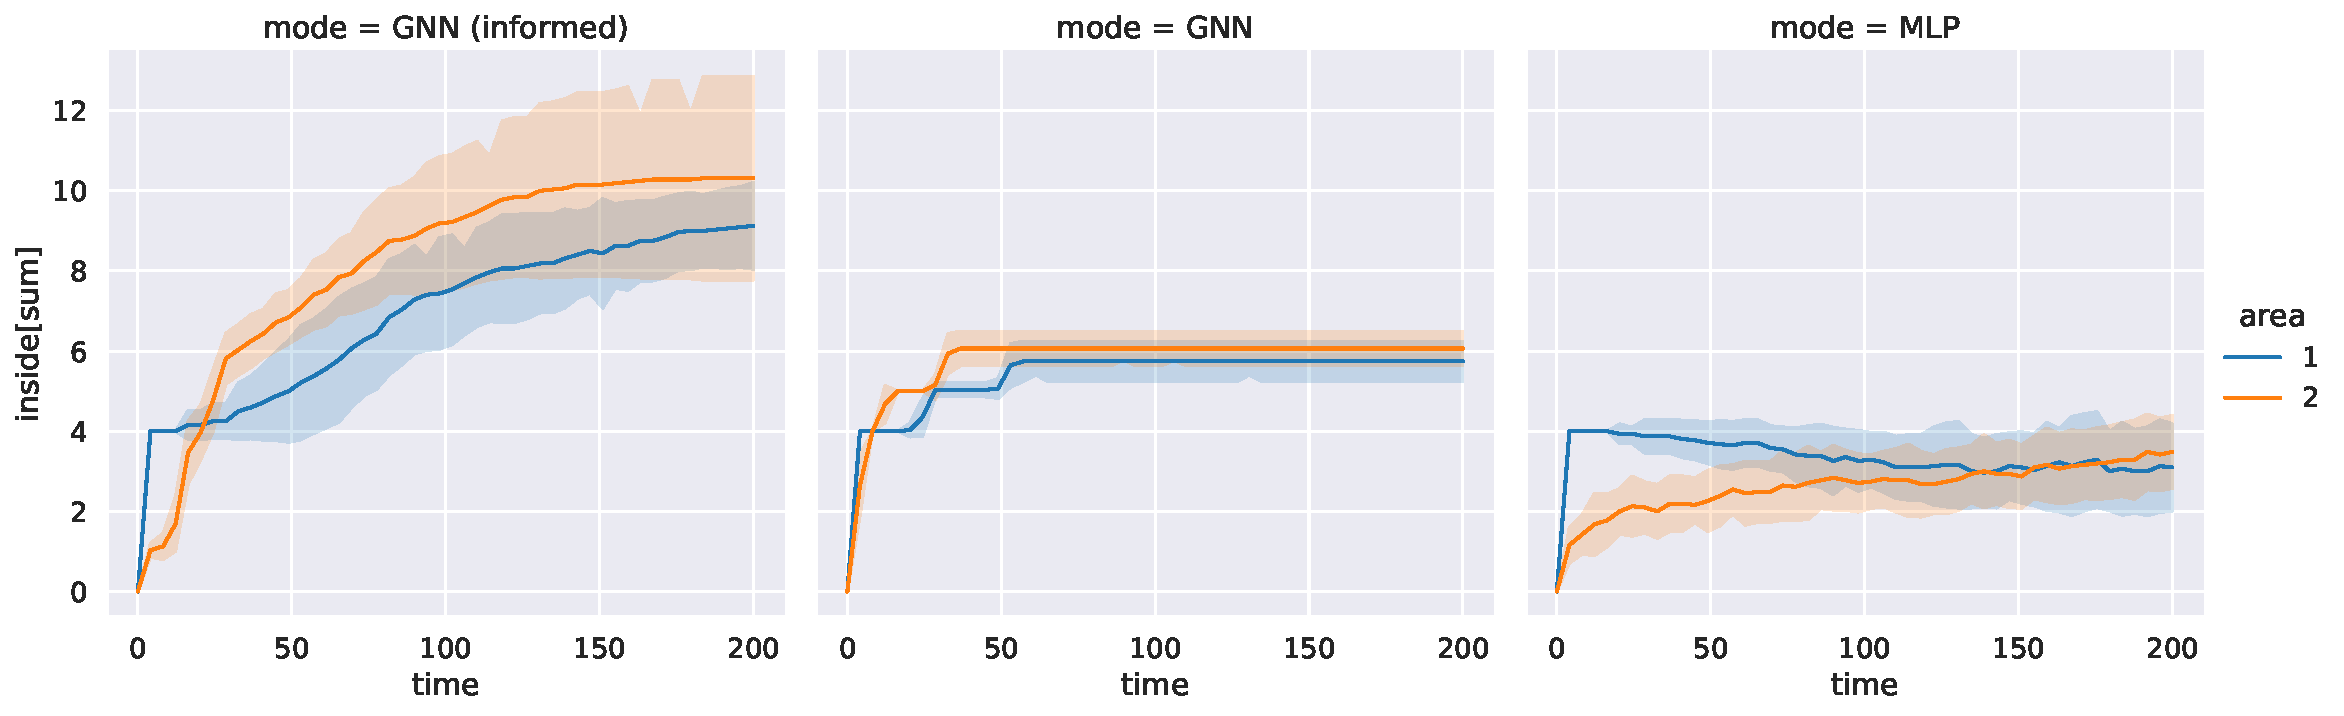
\includegraphics[width=\linewidth]{papers/acsos2023/imgs/inside-two-test}
    \caption{\emph{Two Zones} experiment: aggregated number of drones inside each phenomenon}
    \label{acsos2023:fig:inside-two-test}
  \end{subfigure}
  \begin{subfigure}[b]{0.75\linewidth}
    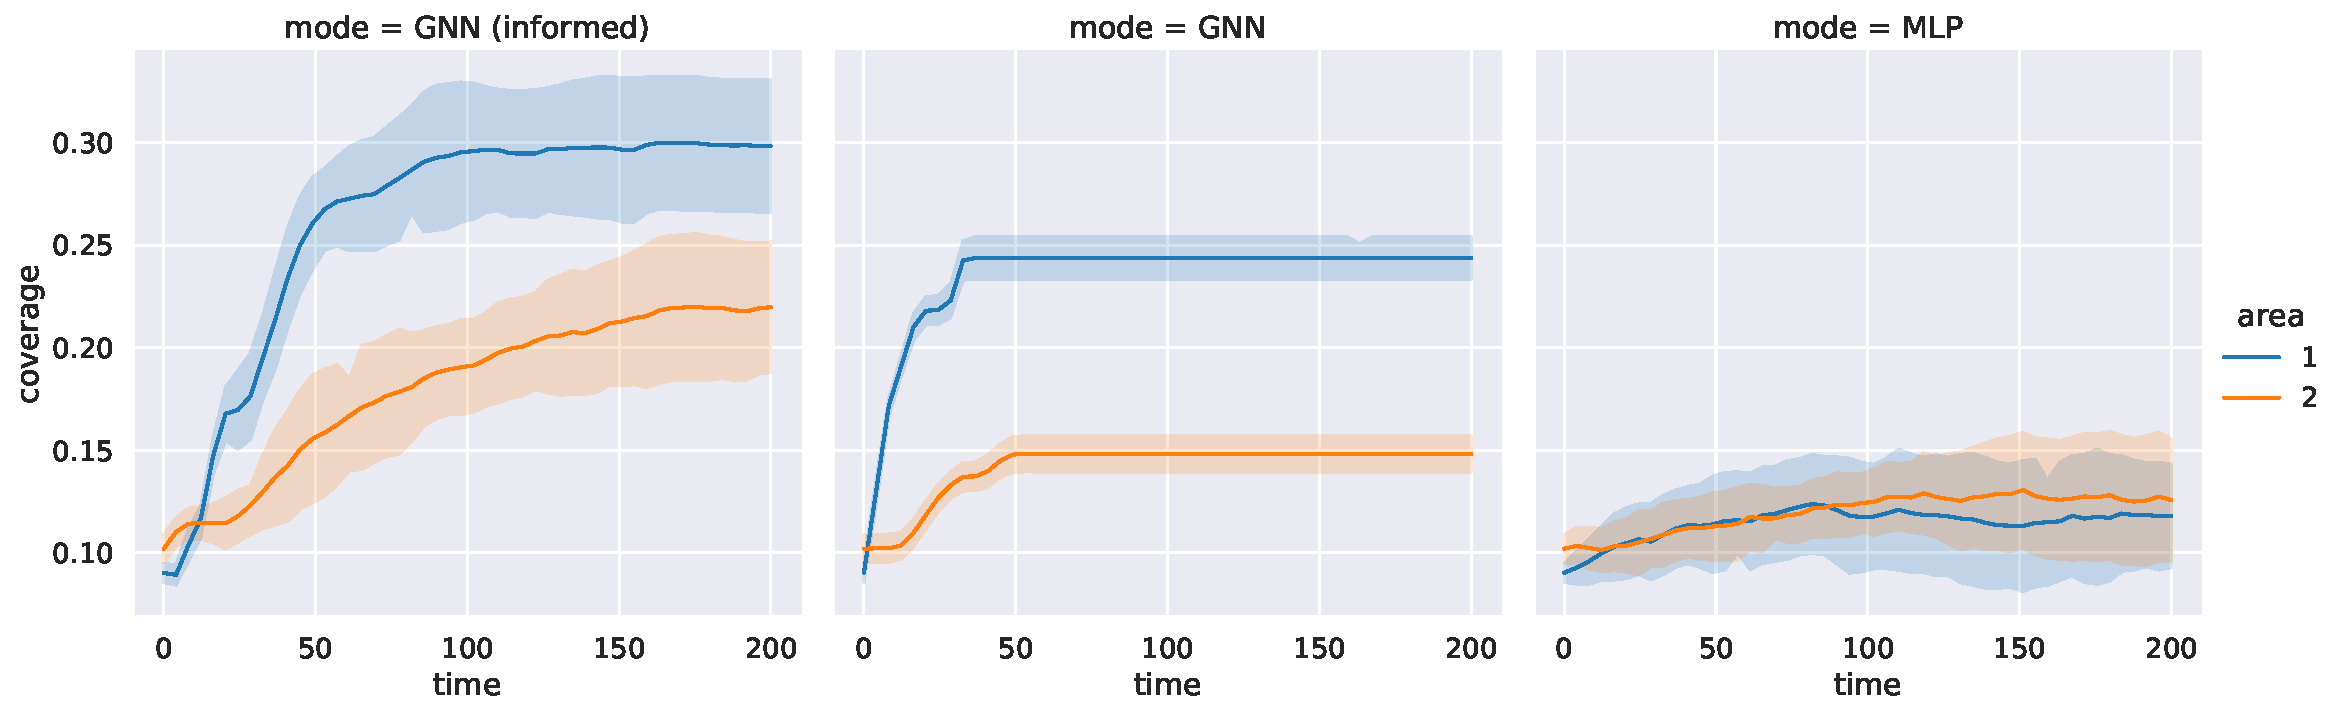
\includegraphics[width=\linewidth]{papers/acsos2023/imgs/coverage-two-test}
    \caption{\emph{Two Zones} experiment: ratio of covered to the uncovered zones both phenomena}
    \label{acsos2023:fig:coverage-two-test}
  \end{subfigure} 
  \caption{Coverage of two zones using the different modes of the controller.}
  \label{acsos2023:fig:resCoverage}
\end{figure*}

\section{Final Remarks}
\label{acsos2023:sec:conclusion}
In this chapter, 
 we have introduced a novel approach for constructing distributed controllers by leveraging aggregate computing to encode agent interactions, 
 along with the combination of \ac{DQN} and \ac{GNN} for synthesizing distributed intelligence.
The proposed \emph{Field-Informed reinforcement learning} (FIRL) approach offers a promising solution to the challenges faced in coordinating multi-agent systems. 
By combining manual design and machine learning techniques, 
 the approach enables agents to autonomously learn and adapt their behaviour while leveraging locally available information. 
%
The demonstrated success in the proposed case study in solving collective tasks underscores the potential impact of this approach in advancing the field of multi-agent systems and swarm robotics. 
%\ga{Page budget: 0.5}